%
% Niniejszy plik stanowi przykład formatowania pracy magisterskiej na
% Wydziale MIM UW.  Szkielet użytych poleceń można wykorzystywać do
% woli, np. formatujac wlasna prace.
%
% Zawartosc merytoryczna stanowi oryginalnosiagniecie
% naukowosciowe Marcina Wolinskiego.  Wszelkie prawa zastrzeżone.
%
% Copyright (c) 2001 by Marcin Woliński <M.Wolinski@gust.org.pl>
% Poprawki spowodowane zmianami przepisów - Marcin Szczuka, 1.10.2004
% Poprawki spowodowane zmianami przepisow i ujednolicenie 
% - Seweryn Karłowicz, 05.05.2006
% Dodanie wielu autorów i tłumaczenia na angielski - Kuba Pochrybniak, 29.11.2016

% dodaj opcję [licencjacka] dla pracy licencjackiej
% dodaj opcję [en] dla wersji angielskiej (mogą być obie: [licencjacka,en])
\documentclass[licencjacka]{pracamgr}

\usepackage{graphicx,xcolor}

% Dane magistranta:
%\autor{Imię Nazwisko}{123456}


% Dane magistrantów:
\autor{Daniel Gutowski}{372207}
\autori{Jakub Kuklis}{371125}
\autorii{Adrian Naruszko}{371233}
\autoriii{Filip Plata}{371335}

\title{????}


%\tytulang{An implementation of a difference blabalizer based on the theory of $\sigma$ -- $\rho$ phetors}

%kierunek: 
% - matematyka, informacyka, ...
% - Mathematics, Computer Science, ...
\kierunek{informatyka}

% informatyka - nie okreslamy zakresu (opcja zakomentowana)
% matematyka - zakres moze pozostac nieokreslony,
% a jesli ma byc okreslony dla pracy mgr,
% to przyjmuje jedna z wartosci:
% {metod matematycznych w finansach}
% {metod matematycznych w ubezpieczeniach}
% {matematyki stosowanej}
% {nauczania matematyki}
% Dla pracy licencjackiej mamy natomiast
% mozliwosc wpisania takiej wartosci zakresu:
% {Jednoczesnych Studiow Ekonomiczno--Matematycznych}

% \zakres{Tu wpisac, jesli trzeba, jedna z opcji podanych wyzej}

% Praca wykonana pod kierunkiem:
% (podać tytuł/stopień imię i nazwisko opiekuna
% Instytut
% ew. Wydział ew. Uczelnia (jeżeli nie MIM UW))
\opiekun{mgr. Krzysztofa Wojciecha Ciebiery\\
  Instytut Informatyki\\
  }

% miesiąc i~rok:
\date{Luty 2018}

%Podać dziedzinę wg klasyfikacji Socrates-Erasmus:
\dziedzina{ 
%11.0 Matematyka, Informatyka:\\ 
%11.1 Matematyka\\ 
%11.2 Statystyka\\ 
11.3 Informatyka\\ 
%11.4 Sztuczna inteligencja\\ 
%11.5 Nauki aktuarialne\\
%11.9 Inne nauki matematyczne i informatyczne
}

%Klasyfikacja tematyczna wedlug AMS (matematyka) lub ACM (informatyka)
\klasyfikacja{D. Software\\
  D.127. Blabalgorithms\\
  D.127.6. Numerical blabalysis \\
  ??TODO
  }

% Słowa kluczowe:
\keywords{blabaliza różnicowa, fetory $\sigma$-$\rho$, fooizm,
  blarbarucja, blaba, fetoryka, baleronik, ??TODO}

% Tu jest dobre miejsce na Twoje własne makra i~środowiska:
\newtheorem{defi}{Definicja}[section]

% koniec definicji

\begin{document}

\maketitle

%tu idzie streszczenie na strone poczatkowa
\begin{abstract}
  W~pracy przedstawiamy opis współpracy w firmą e-point.
  Produktem rozwijanym przez tą firmę jest autorski
  system CMS. Na chwilę obecną ma on architekturę monolitu.
  Naszym zadaniem było napisanie mikroserwisów umożliwiających
  dalszą modernizację i modularyzację tego produktu.
\end{abstract}

\tableofcontents
%\listoffigures
%\listoftables

\chapter*{Wprowadzenie}
\addcontentsline{toc}{chapter}{Wprowadzenie}

Początkowo mieliśmy zrealizować inny projekt - kategoryzację
użytkowników na podstawie aktywności na stronach internetowych. Zdążyliśmy zaimplementować
podstawową architekturę, a także skonfigurować narzędzia deweloperskie na AWS.
Niestety, nastąpiła zmiana projektu wymuszona okolicznościami zewnętrznymi na
realizację pierwszego etapu modernizacji produktu e-pointu na nowe
technologie oraz architekturę.

Zajmowaliśmy się implementacją dwóch mikroserwisów:
\begin{enumerate}
\item Element integrujący między bazą danych aktualnego CMSa a nowym mechanizmem renderingu.
	Jest to RESTowa aplikacja udostępniająca niektóre dane z bazy danych potrzebne modułowi renderingu.
\item Nowy mechanizm renderujący strony wraz z rejestrami usług. Gdzie przez usługi rozumiane są
	kroki/akcje wykonywane w trakcie tworzenia strony. Np. podmiana tagów, (??TODO). W docelowej architekturze
	mają to być niezależne mikroserwisy.
\end{enumerate}


\chapter{Opis modernizacji architektury}


\section{Dotychczasowy monolit}
Do tej pory jedna aplikacja(a.k.a. ACN) obsługiwała zapytania HTTP od momentu pojawienia się do końcowego serwowania strony WWW.
Taka struktura powoduje skomplikowanie kodu, utrudnia wprowadzanie zmian a w przypadku awarii serwisu komplikuje lokalizację błędu.

\begin{figure}\label{architektura}
	\centering
	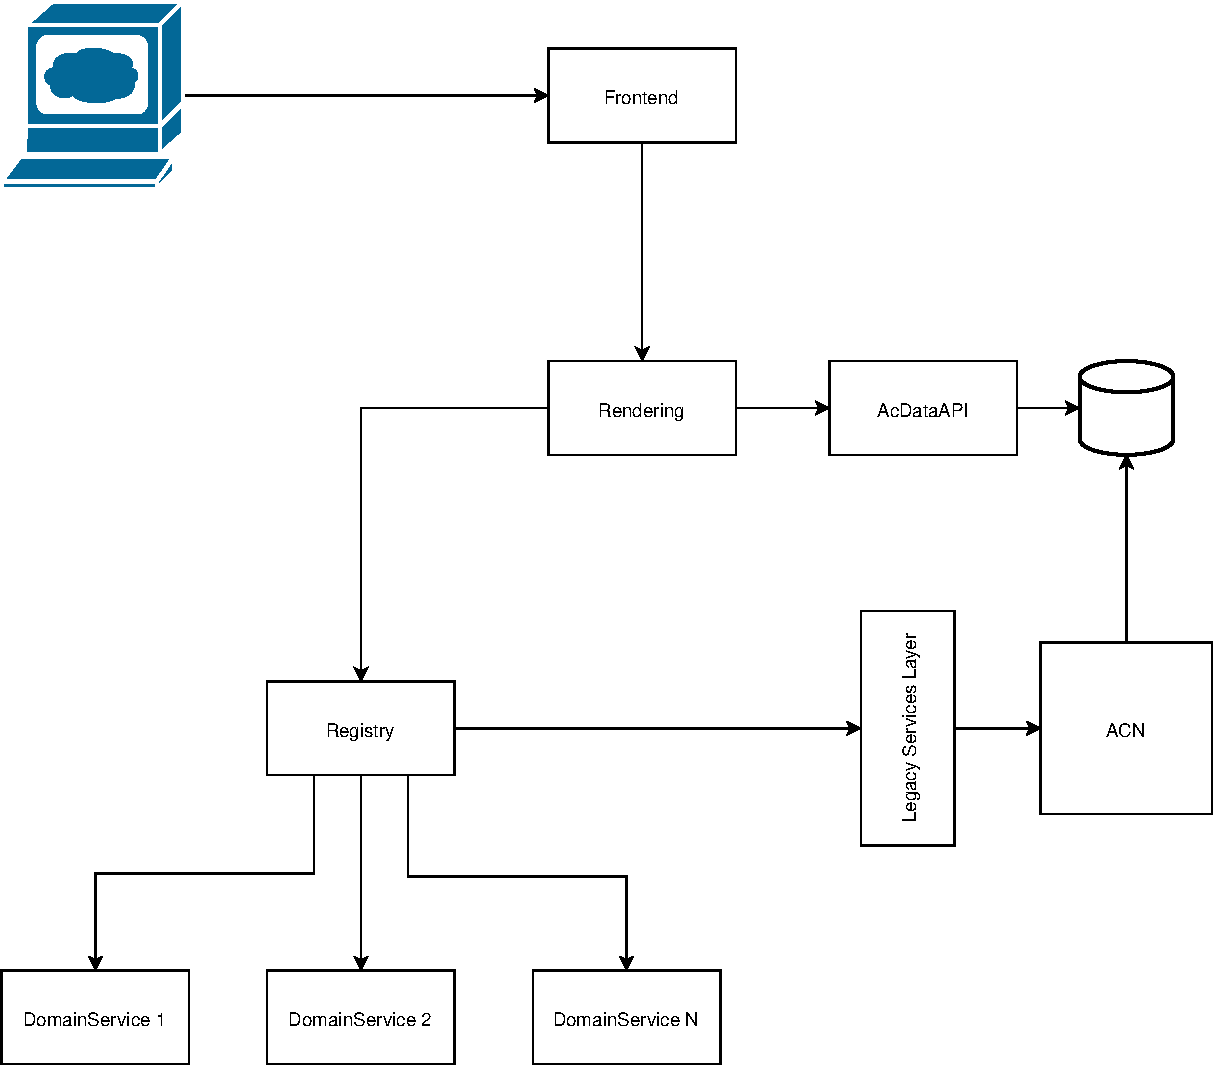
\includegraphics[scale=0.82]{architecture.pdf}
	\caption{Schemat wydzielonych aplikacji}
\end{figure}

\section{Nowa architektura}
Rozwiązanie zaproponowane przez firmę i wdrażane przez nas to rozdzielenie czynności wykonywanych w ACN na kilka mikroserwisów RESTowych.
Jak widać na rysunku \ref{architektura} wydzielone zostały następujące aplikacje:
\begin{itemize}
\item Frontend - przyjmowanie zapytań i serwowanie stron WWW
\item Rendering - tworzenie stron na podstawie szablonów, wykorzystuje usługi udostępniane przez registry
\item AcDataAPI - abstrakcja bazy danych, udostępnia tylko niezbędne renderingowi dane
\item Registry - rejestr usług tj. podmiana tagów, personalizacja treści itp.
\item ACN - dotychczasowa aplikacja implementująca niektóre usługi, w końcowym etapie ma zniknąć
\end{itemize}
W tej pracy opisujemy naszą pracę nad renderingiem i dataAPI.


\chapter{Implementacja elementu integrującego z bazą danych}


\section{Użyte technologie}
\begin{enumerate}
\item JAVA w wersji 8
\item Spring - framework do tworzenia aplikacji Javowych
\item Jooq(Java Object Oriented Querying) - lekka biblioteka do mapowania baz danych.
	Posiadającą funkcję generowania klas Javy na podstawie bazy danych
\item Redis - wykorzystany do cachowania wyników zapytań
\item Elastic Stack - Logstash, Metricbeat, ElasticSearch i Kibana użyte do monitorowania aplikacji
\item Gatling - framework do tworzenia i wykonywania scenariuszy testów wdajnościowych
\item Docker - uruchamianie aplikacji w kontenerze
\end{enumerate}


\section{Założenia aplikacji}
\begin{enumerate}
\item Aplikacja ma specyfikować oraz implementować kontrakt będący endpointami RESTowymi.
	Odpowiedzią na dane zapytanie jest JSON zawierający dane z bazy danych.
	Nazwy endpointów składają się z wersji API oraz nazwy.
	Np. \emph{/v1/language-version} 
\item Odpowiedzi na zapytania mają być cachowane. Inwalidacja ??TODO
\item Częścią projektu jest napisanie testów poprawnościowych i wydajnościowych.
\end{enumerate}


\section{Iteracja 1}
Wstępnie zrealizowany przykład oparcia rozwiązania w sposób bardzo
bezpośrednio o pakiet Jooq został odrzucony po zaprezentowaniu
przykładowej implementacji ze względu na ujawnione braki w
architekturze rozwiązania.
Ujawniła się konieczność zapewnienia ścisłego kontraktu 
poprzez API, mimo zmian schematu bazy danych z której
pobierane są dane.

Zwłaszcza nad tą fazą projektu trwała najdłuższa dyskusja oraz analiza
dostępnych narzędzi. Po rozpatrzeniu możliwości zaprezentowanych
kawałkami kodu, osoba odpowiedzialna za projekt z e-pointu
zdecydowała się właśnie na pakiet Jooq w połączeniu
z generacją klas na podstawie aktualnego stanu bazy danych, wydzielając
jednak warstwę zależną od Jooq od reszty kodu, który nie zależy od sposobu
dostępu do bazy danych.

Do monitorowania aktywnych instancji aplikacji użyliśmy gotowego, dedykowanego narzędzia 
spring-boot-admin. Niestety okazało się że konfiguracja jest równie łatwa co ograniczona i 
nie spełnia wymogów postawionych przez klienta.


\section{Iteracja 2}
Do realizacji zatem przyjęliśmy architekturę z kilkoma
warstwami pośredniczącymi, każda wykonuje oddzielne zadania.
I tak zaczynając od warstwy najbliżej bazy danych:

\begin{enumerate}
\item Umożliwia dostęp do bazy poprzez Jooqa
\item Zajmuje się sprawą podzielenia danych klientów na schematy w bazie danych
	(zarządzanie aktualnym schematem)
\item Ukrywa Jooq poprzez obiekty domenowe
\item Umożliwia zapewnienie kontraktu kompatybilnego wstecz pomimo zmian schematu bazy danych
\end{enumerate}

Ostatni punkt zapewniony jest przez wersjonowanie API pakietami java, z
wydzielonym wspólnym kodem - czyli zdecydowaną większością.

Konfiguracja cache sprowadzała się dodania kilku adnotacji w kodzie oraz konfiguracji Redisa.

Tym razem do monitorowania instancji aplikacji skorzystaliśmy z Elastic Stacka, który co prawda wymaga 
ręcznego wprowadzenia zasad dla wymaganych statystyk, ale w zamian daje możliwość niemalże dowolnej ich
konfiguracji.

Kolejnym wymaganiem klienta było przeprowadzenie testów wydajnościowych 
zaproponowanego rozwiązania. W tym celu napisaliśmy scenariusze korzystając 
z frameworku Gatling napisanego w Scali. 







\if{false}
Pojęciem pierwotnym blabalii fetorycznej jest \emph{blaba}.
Blabaliści nie podają jego definicji, mówiąc za Ciach-Pfe t-\=am
K\^un (fooistyczny mędrzec, XIX w. p.n.e.):
\begin{quote}
  Blaba, który jest blaba, nie jest prawdziwym blaba.

\raggedleft\slshape tłum. z~chińskiego Robert Blarbarucki
\end{quote}

\section{Definicje}

Oto dwie definicje wprowadzające podstawowe pojęcia blabalii
fetorycznej:

\begin{defi}\label{skupienie}
  Silny, zwarty i gotowy fetor bazowy nazwiemy \emph{skupieniem}.
\end{defi}

\begin{defi}\label{fetor}
  \emph{Fetorem} nazwiemy skupienie blaba spełniające następujący
  \emph{aksjomat reperkusatywności}:
  $$\forall \mathcal{X}\in Z(t)\ \exists
  \pi\subseteq\oint_{\Omega^2}\kappa\leftrightarrow 42$$
\end{defi}


\section{Blabalizator różnicowy}

Teoretycy blabalii (zob. np. pracę~\cite{grglo}) zadowalają się
niekonstruktywnym opisem natury fetorów.

Podstawowym narzędziem blabalii empirycznej jest blabalizator
różnicowy.  Przyrząd ten pozwala w~sposób przybliżony uzyskać
współczynniki rozkładu Głombaskiego dla fetorów bazowych
i~harmonicznych.  Praktyczne znaczenie tego procesu jest oczywiste:
korzystając z~reperkusatywności pozwala on przejść do przestrzeni
$\Lambda^{\nabla}$, a~tym samym znaleźć retroizotonalne współczynniki
semi-quasi-celibatu dla klatek Rozkoszy (zob.~\cite{JR}).

Klasyczne algorytmy dla blabalizatora różnicowego wykorzystują:
\begin{enumerate}
\item dualizm falowo-korpuskularny, a w szczególności
  \begin{enumerate}
  \item korpuskularną naturę fetorów,
  \item falową naturę blaba,
  \item falowo-korpuskularną naturę gryzmołów;
  \end{enumerate}
\item postępującą gryzmolizację poszczególnych dziedzin nauki, w
  szczególności badań systemowych i rozcieńczonych;
\item dynamizm fazowy stetryczenia parajonizacyjnego;
\item wreszcie tradycyjne opozycje:
  \begin{itemize}
  \item duch --- bakteria,
  \item mieć --- chcieć,
  \item myśl --- owsianka,
  \item parafina --- durszlak\footnote{Więcej o tym przypadku --- patrz
      prace Gryzybór-Głombaskiego i innych teoretyków nurtu
      teoretyczno-praktycznego badań w~Instytucie Podstawowych
      Problemów Blabalii w~Fifie.},
  \item logos --- termos%\footnote{Szpotański}
  \end{itemize}
  z właściwym im przedziwym dynamizmem.
\end{enumerate}

\begin{figure}[tp]
  \centering
  \framebox{\vbox to 4cm{\vfil\hbox to
      7cm{\hfil\tiny.\hfil}\vfil}}
  \caption{Artystyczna wizja blaba w~obrazie węgierskiego artysty
    Josipa~A. Rozkoszy pt.~,,Blaba''}
\end{figure}

\chapter{Wcześniejsze implementacje blabalizatora
  różnicowego}\label{r:losers}

\section{Podejście wprost}

Najprostszym sposobem wykonania blabalizy jest siłowe przeszukanie
całej przestrzeni rozwiązań.  Jednak, jak łatwo wyliczyć, rozmiar
przestrzeni rozwiązań rośnie wykładniczo z~liczbą fetorów bazowych.
Tak więc przegląd wszystkich rozwiązań sprawdza się jedynie dla bardzo
prostych przestrzeni lamblialnych.  Oznacza to, że taka metoda ma
niewielkie znaczenie praktyczne --- w~typowym przypadku z~życia trzeba
rozważać przestrzenie lamblialne wymiaru rzędu 1000.

W~literaturze można znaleźć kilka prób opracowania heurystyk dla
problemu blabalizy (por. \cite{heu}).  Korzystając z~heurystyk daje
się z~pewnym trudem dokonać blabalizy w~przestrzeni o~np.~500 fetorach
bazowych.  Należy jednak pamiętać, że heurystyka nie daje gwarancji
znalezienia najlepszego rozwiązania.  Fifak w~pracy~\cite{ff-sr}
podaje, jak dla dowolnie zadanej funkcji oceniającej skonstruować
dane, dla których rozwiązanie wygenerowane przez algorytm heurystyczny
jest dowolnie odległe od rzeczywistego.

\section{Metody wykorzystujące teorię Głombaskiego}

Teoria Głombaskiego (zob.~\cite{grglo}) dostarcza eleganckiego
narzędzia opisu przejścia do przestrzeni $\Lambda^{\nabla}$.
Wystarczy mianowicie przedstawić fetory bazowe wyjściowej przestrzeni
lamblialnej w~nieskończonej bazie tak zwanych wyższych aromatów.
(Formalną definicję tego pojęcia przedstawię w~rozdziale poświęconym
teorii Fifaka).  Podstawową cechą wyższych aromatów jest ulotność.  To
zaś oznacza, że odpowiednio dobierając współczynniki przejścia do
przestrzeni wyższych aromatów można zagwarantować dowolną z~góry
zadaną dokładność przybliżonego rozwiązania problemu blabalizy.

Oczywiście ze względu na nieskończony wymiar przestrzeni wyższych
aromatów koszt poszukiwania współczynników blabalizy jest liniowy ze
względu na wymiar wyjściowej przestrzeni lamblialnej.

\section{Metody wykorzystujące własności fetorów $\sigma$}

Najchętniej wykorzystywaną przestrzenią wyższych aromatów jest
przestrzeń fetorów~$\sigma$.  Fetory $\sigma$ dają szczególnie prostą
bazę podprzestrzeni widłowej.  Wiąże się to z~faktem, że w~tym przypadku
fetory harmoniczne wyższych rzędów są pomijalne (rzędu $2^{-t^3}$,
gdzie $t$ jest wymiarem wyjściowej przestrzeni lamblialnej).

Niestety z~fetorami $\sigma$ wiąże się też przykre ograniczenie: można
wykazać (zob.~\cite[s. 374]{ff-sr}), że dla dowolnie dobranej bazy
w~podprzestrzeni widłowej istnieje ograniczenie dolne w~metryce sierpa
na odległość rzutu dokładnego rozwiązania problemu blabalizy na
podprzestrzeń widłową.  Ponieważ rzut ten stanowi najlepsze
przybliżone rozwiązanie, jakie można osiągnąć nie naruszając aksjomatu
reperkusatywności, więc istnieje pewien nieprzekraczalny próg
dokładności dla blabalizy wykonanej przez przejście do przestrzeni
fetorów $\sigma$.  Wartość retroinicjalną tego progu nazywa się
\textit{reziduum blabicznym}.

\chapter{Teoria fetorów $\sigma$-$\rho$}\label{r:fifak}

Głównym odkryciem Fifaka jest, że fetor suprakowariantny może
gryzmolizować dowolny ideał w~podprzestrzeni widłowej przestrzeni
lamblialnej funkcji Rozkoszy.

Udowodnienie tego faktu wymagało wykorzystania twierdzeń pochodzących
z~kilku niezależnych teorii matematycznych (zob. na przykład:
\cite{russell,spyrpt,JR,beaman,hopp,srinis}).  Jednym z~filarów
dowodu jest teoria odwzorowań owalnych Leukocyta (zob.~\cite{leuk}).

Znaczenie twierdzenia Fifaka dla problemu blabalizy polega na tym, że
znając retroizotonalne współczynniki dla klatek Rozkoszy można
przeprowadzić fetory bazowe na dwie nieskończone bazy fetorów $\sigma$
w~przestrzeni $K_7$ i~fetorów $\rho$ w~odpowiedniej
quasi-quasi-przestrzeni równoległej (zob.~\cite{hopp}).  Zasadnicza
różnica w~stosunku do innych metod blabalizy polega na tym, że
przedstawienie to jest dokładne.

\chapter{Dokumentacja użytkowa i~opis implementacji}\label{r:impl}

Program przygotowany dla systemu operacyjnego M\$ Windows uruchamia
się energicznym dwumlaskiem na jego ikonce w~folderze
\verb+\\FIDO\FOO\BLABA+.  Następnie kolistym ruchem ręki należy
naprowadzić kursor na menu \texttt{Blabaliza} i~uaktywnić pozycję
\texttt{Otwórz plik}.  Po wybraniu pliku i~zatwierdzeniu wyboru
przyciskiem \texttt{OK} rozpocznie się proces blabalizy.  Wyniki
zostaną zapisane w~pliku o~nazwie \texttt{99-1a.tx.43} w~bieżącym
folderze.

\chapter{Podsumowanie}

W~pracy przedstawiono pierwszą efektywną implementację blabalizatora
różnicowego.  Umiejętność wykonania blabalizy numerycznej dla danych
,,z życia'' stanowi dla blabalii fetorycznej podobny przełom, jak dla
innych dziedzin wiedzy stanowiło ogłoszenie teorii Mikołaja Kopernika
i~Gryzybór Głombaskiego.  Z~pewnością w~rozpocznynającym się XXI wieku
będziemy obserwować rozkwit blabalii fetorycznej.

Trudno przewidzieć wszystkie nowe możliwości, ale te co bardziej
oczywiste można wskazać już teraz.  Są to:
\begin{itemize}
\item degryzmolizacja wieńców telecentrycznych,
\item realizacja zimnej reakcji lambliarnej,
\item loty celulityczne,
\item dokładne obliczenie wieku Wszechświata.
\end{itemize}

\section{Perspektywy wykorzystania w~przemyśle}

Ze względu na znaczenie strategiczne wyników pracy ten punkt uległ
utajnieniu.

\appendix

\chapter{Główna pętla programu zapisana w~języku T\=oFoo}

\begin{verbatim}
[[foo]{,}[[a3,(([(,),{[[]]}]),
  [1; [{,13},[[[11],11],231]]].
  [13;[!xz]].
  [42;[{,x},[[2],{'a'},14]]].
  [br;[XQ*10]].
 ), 2q, for, [1,]2, [..].[7]{x}],[(((,[[1{{123,},},;.112]],
        else 42;
   . 'b'.. '9', [[13141],{13414}], 11),
 [1; [[134,sigma],22]].
 [2; [[rho,-],11]].
 )[14].
 ), {1234}],]. [map [cc], 1, 22]. [rho x 1]. {22; [22]},
       dd.
 [11; sigma].
        ss.4.c.q.42.b.ll.ls.chmod.aux.rm.foo;
 [112.34; rho];
        001110101010101010101010101010101111101001@
 [22%f4].
 cq. rep. else 7;
 ]. hlt
\end{verbatim}

\chapter{Przykładowe dane wejściowe algorytmu}

\begin{center}
  \begin{tabular}{rrr}
    $\alpha$ & $\beta$ & $\gamma_7$ \\
    901384 & 13784 & 1341\\
    68746546 & 13498& 09165\\
    918324719& 1789 & 1310 \\
    9089 & 91032874& 1873 \\
    1 & 9187 & 19032874193 \\
    90143 & 01938 & 0193284 \\
    309132 & $-1349$ & $-149089088$ \\
    0202122 & 1234132 & 918324098 \\
    11234 & $-109234$ & 1934 \\
  \end{tabular}
\end{center}

\chapter{Przykładowe wyniki blabalizy
    (ze~współczynnikami~$\sigma$-$\rho$)}

\begin{center}
  \begin{tabular}{lrrrr}
    & Współczynniki \\
    & Głombaskiego & $\rho$ & $\sigma$ & $\sigma$-$\rho$\\
    $\gamma_{0}$ & 1,331 & 2,01 & 13,42 & 0,01 \\
    $\gamma_{1}$ & 1,331 & 113,01 & 13,42 & 0,01 \\
    $\gamma_{2}$ & 1,332 & 0,01 & 13,42 & 0,01 \\
    $\gamma_{3}$ & 1,331 & 51,01 & 13,42 & 0,01 \\
    $\gamma_{4}$ & 1,332 & 3165,01 & 13,42 & 0,01 \\
    $\gamma_{5}$ & 1,331 & 1,01 & 13,42 & 0,01 \\
    $\gamma_{6}$ & 1,330 & 0,01 & 13,42 & 0,01 \\
    $\gamma_{7}$ & 1,331 & 16435,01 & 13,42 & 0,01 \\
    $\gamma_{8}$ & 1,332 & 865336,01 & 13,42 & 0,01 \\
    $\gamma_{9}$ & 1,331 & 34,01 & 13,42 & 0,01 \\
    $\gamma_{10}$ & 1,332 & 7891432,01 & 13,42 & 0,01 \\
    $\gamma_{11}$ & 1,331 & 8913,01 & 13,42 & 0,01 \\
    $\gamma_{12}$ & 1,331 & 13,01 & 13,42 & 0,01 \\
    $\gamma_{13}$ & 1,334 & 789,01 & 13,42 & 0,01 \\
    $\gamma_{14}$ & 1,331 & 4897453,01 & 13,42 & 0,01 \\
    $\gamma_{15}$ & 1,329 & 783591,01 & 13,42 & 0,01 \\
  \end{tabular}
\end{center}

\begin{thebibliography}{99}
\addcontentsline{toc}{chapter}{Bibliografia}

\bibitem[Bea65]{beaman} Juliusz Beaman, \textit{Morbidity of the Jolly
    function}, Mathematica Absurdica, 117 (1965) 338--9.

\bibitem[Blar16]{eb1} Elizjusz Blarbarucki, \textit{O pewnych
    aspektach pewnych aspektów}, Astrolog Polski, Zeszyt 16, Warszawa
  1916.

\bibitem[Fif00]{ffgg} Filigran Fifak, Gizbert Gryzogrzechotalski,
  \textit{O blabalii fetorycznej}, Materiały Konferencji Euroblabal
  2000.

\bibitem[Fif01]{ff-sr} Filigran Fifak, \textit{O fetorach
    $\sigma$-$\rho$}, Acta Fetorica, 2001.

\bibitem[Głomb04]{grglo} Gryzybór Głombaski, \textit{Parazytonikacja
    blabiczna fetorów --- nowa teoria wszystkiego}, Warszawa 1904.

\bibitem[Hopp96]{hopp} Claude Hopper, \textit{On some $\Pi$-hedral
    surfaces in quasi-quasi space}, Omnius University Press, 1996.

\bibitem[Leuk00]{leuk} Lechoslav Leukocyt, \textit{Oval mappings ab ovo},
  Materiały Białostockiej Konferencji Hodowców Drobiu, 2000.

\bibitem[Rozk93]{JR} Josip A.~Rozkosza, \textit{O pewnych własnościach
    pewnych funkcji}, Północnopomorski Dziennik Matematyczny 63491
  (1993).

\bibitem[Spy59]{spyrpt} Mrowclaw Spyrpt, \textit{A matrix is a matrix
    is a matrix}, Mat. Zburp., 91 (1959) 28--35.

\bibitem[Sri64]{srinis} Rajagopalachari Sriniswamiramanathan,
  \textit{Some expansions on the Flausgloten Theorem on locally
    congested lutches}, J. Math.  Soc., North Bombay, 13 (1964) 72--6.

\bibitem[Whi25]{russell} Alfred N. Whitehead, Bertrand Russell,
  \textit{Principia Mathematica}, Cambridge University Press, 1925.

\bibitem[Zen69]{heu} Zenon Zenon, \textit{Użyteczne heurystyki
    w~blabalizie}, Młody Technik, nr~11, 1969.

\end{thebibliography}

\fi

\end{document}


%%% Local Variables:
%%% mode: latex
%%% TeX-master: t
%%% coding: latin-2
%%% End:
